\chapter{A New Framework}

The development of Quantum Field Theory was driven by the need to reconcile the principles of quantum mechanics with those of special relativity. Special relativity describes the structure of spacetime and the behavior of objects moving at high velocities, while quantum mechanics governs the behavior of particles at microscopic scales. However, neither theory alone could adequately describe phenomena involving both high energies and small distances, such as particle creation and annihilation.

Quantum mechanics does not include relativistic effects:
\begin{itemize}
    \item The concept of a \textbf{limiting speed is absent}.
    \item The \textbf{energy expression} for a free particle is incompatible with the relativistic one:\\
    $E_{\text{QM}} = \frac{p^2}{2m}$ instead of $E_{\text{SR}} = \sqrt{p^2c^2 + m^2c^4}$.
\end{itemize}

Special relativity, on the other hand, does not incorporate quantum principles:
\begin{itemize}
    \item It does not account for \textbf{quantization} of physical observables, such as energy.
    \item The \textbf{promotion of observables to operators} acting on a Hilbert space is missing.
\end{itemize}

\begin{figure}[H]
\centering
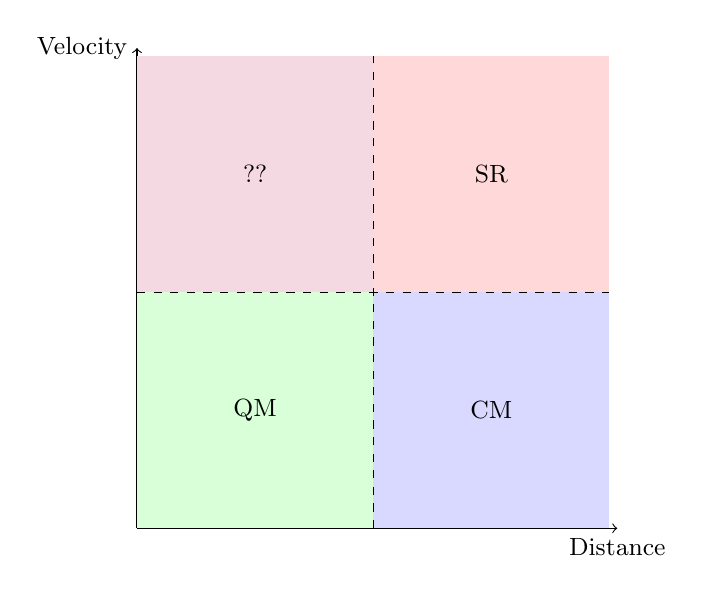
\begin{tikzpicture}[scale=1, font=\small]

\draw[->] (0,0) -- (6.1,0) node[anchor=north] {Distance};
\draw[->] (0,0) -- (0,6.1) node[anchor=east] {Velocity};

\node at (5.8,-0.3) {};
\node at (0.8,-0.3) {};
\node[rotate=90] at (-0.3,5.8) {};
\node[rotate=90] at (-0.3,0.8) {};

\fill[blue!15] (3,0) rectangle (6,3);
\node at (4.5,1.5) {CM};

\fill[green!15] (0,0) rectangle (3,3);
\node at (1.5,1.5) {QM};

\fill[red!15] (3,3) rectangle (6,6);
\node at (4.5,4.5) {SR};

\fill[purple!15] (0,3) rectangle (3,6);
\node[text=black] at (1.5,4.5) {??};

\draw[dashed] (3,0)--(3,6);
\draw[dashed] (0,3)--(6,3);

\end{tikzpicture}
\caption{Schematic diagram of the four fundamental regimes of physics.}
\end{figure}

We need a new framework to describe the regime of small distances and high velocities, where both quantum and relativistic effects are significant. The idea to overcome the shown limitations is to use expressions from SR and incorporate them into a quantum framework: a \textbf{relativistic quantum mechanics} theory.

\section{Relativistic Quantum Mechanics and its Limitations}

The first attempt to construct a relativistic quantum theory was to modify the Schrödinger equation by replacing the non-relativistic energy-momentum relation with the relativistic one. We are basically in a quantum framework:
\begin{itemize}
    \item Observables are promoted to operators acting on a Hilbert space by imposing \textit{canonical commutation relations}:\\
    $[\hat{\mathbf{x}}, \hat{\mathbf{p}}] = i\hbar \implies \hat{\mathbf{p}} = -i\hbar \frac{\mathrm{d}}{\mathrm{d}\mathbf{x}},\quad [\hat{t}, \hat{H}] = i\hbar \implies \hat{H} = i\hbar \frac{\mathrm{d}}{\mathrm{d}t}$.
    \item Operators act on a Hilbert space $\mathcal{H}$, where its states represent physical states of the system, with a \textbf{fixed number of particles}.
    \item Eigenvectors of a complete set of commuting observables form a basis for the Hilbert space; the eigenvalues correspond to the possible measurement outcomes:\\ 
    \(\hat{\mathbf{p}} \ket{p} = p \ket{p}, \quad \int \mathrm{d}p \ket{p}\bra{p} = 1\).
    \item The time evolution of states is governed by the \textbf{generalized Schrödinger equation}: $-i\hbar \frac{\partial}{\partial t} \psi(\mathbf{x}, t) = \hat{H} \psi(\mathbf{x}, t) = \sqrt{\hat{\mathbf{p}}^2c^2 + m^2c^4} \psi(\mathbf{x}, t)$ .
\end{itemize}

However, this approach leads to several issues: it cannot account for particle creation and annihilation, which are essential in relativistic contexts. Additionally, the theory struggles with maintaining causality and Lorentz invariance, and predicts an infinite number of negative energy states, leading to an unstable vacuum.

\subsection*{Production/Annihilation of Particles}

A picture in which the number of particles is fixed cannot describe processes where particles are created or destroyed, such as in high-energy collisions (LHC or other particle colliders) or in nuclear decays.

If we consider a particle with mass $m$ at rest, its energy is given by $E = mc^2$. If we now add an energy to the system, as the particle acquires momentum, its mass becomes negligible and the system is energetically favorable to create new particles. But in order to preserve physical quantities such as charge, lepton number, baryon number, etc., particles must be created in pairs.

\paragraph{Example: particle in a box.} Consider a particle of mass $m$ confined in a three-dimensional box of length $L$. The \textit{Heisenberg uncertainty principle} states that the uncertainty in position $\Delta x$ and the uncertainty in momentum $\Delta p$ satisfy the relation $\Delta x \Delta p \geq \frac{\hbar}{2}$. For a particle confined in a box, we can estimate $\Delta x \sim L$, leading to an uncertainty in momentum of at least $\Delta p \sim \frac{2\hbar}{L}$. If we take the particle to the ultrarelativistic regime,\footnote{In the ultrarelativistic regime, the particle's kinetic energy is much greater than its rest mass energy: \(E^2 = p^2c^2 + m^2c^4 \approx p^2c^2\).} its energy can be approximated as \(E \approx pc\). Therefore, the uncertainty in energy will be:
\[
    \Delta E \geq \frac{2\hbar c}{L}.
\]
If we want to avoid the production of particle-antiparticle pairs, we must ensure that the energy uncertainty is less than the energy required to create such a pair, which is \(2mc^2\). But if we decrease the size of the box \(L\) to increase the precision in position, we increase the uncertainty in energy.
\[
    2mc^2 = \frac{2\hbar c}{L} \implies L = \frac{\hbar}{mc} = \lambda_c.
\]
Here, \(\lambda_c\) is the Compton wavelength of the particle, representing a fundamental limit to the precision with which we can localize a particle without inducing pair production. If we try to confine the particle within a region smaller than its Compton wavelength, the energy uncertainty becomes sufficient to create particle-antiparticle pairs, making it impossible to describe the system with a fixed number of particles.

We need a framework that allows for a variable number of particles, accommodating the creation and annihilation processes inherent in relativistic quantum phenomena (as we will see, a Fock space formalism is required: \(\mathcal{F} = \bigoplus_{n} \mathcal{H}_n\)).

\subsection*{Violation of Causality}

In order to be consistent with special relativity, a physical theory must respect the principle of causality, which states that cause precedes effect and that information cannot travel faster than the speed of light. In relativistic quantum mechanics, the wavefunction can exhibit non-local behavior, leading to potential violations of causality.

To start, let's consider a free particle in the position eigenstate \(\ket{\mathbf{x}}\). The time evolution of the wavefunction is given by the operator \(e^{-\frac{i}{\hbar}Ht}\). Now we can compute the amplitude for finding the particle at a different position \(\mathbf{y}\) after a time \(t\):
\[
    A_{\mathbf{x} \to \mathbf{y}}(t) = \bra{\mathbf{y}}e^{-\frac{i}{\hbar}Ht}\ket{\mathbf{x}}.
\]
We will show that this amplitude is non-zero even when the distance \(|\mathbf{y} - \mathbf{x}|\) is greater than \(ct\), which implies that the particle can be found outside the light cone, violating causality. This is true using QM as well as RQM, in the latter case the effect being less pronounced but still non-zero.

\begin{center}
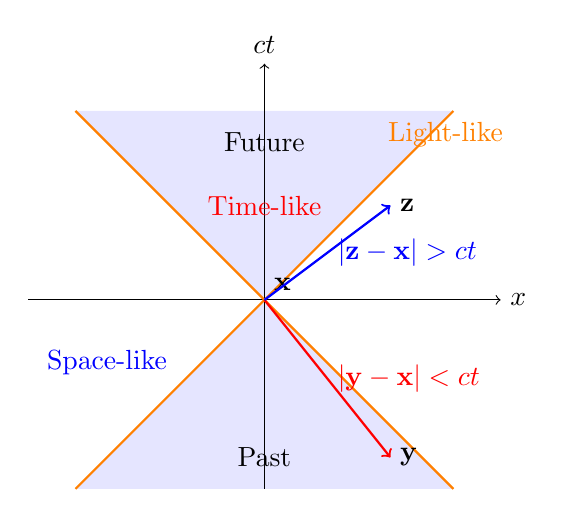
\begin{tikzpicture}[scale=2]

    % Shaded regions (light cone)
    \fill[blue!10] (-1.2,1.2) -- (1.2,1.2) -- (0,0) -- cycle; % future
    \fill[blue!10] (-1.2,-1.2) -- (1.2,-1.2) -- (0,0) -- cycle; % past

    % Axes
    \draw[->] (0,-1.2) -- (0,1.5) node[above] {$ct$};
    \draw[->] (-1.5,0) -- (1.5,0) node[right] {$x$};

    % Light cone lines
    \draw[thick,orange] (-1.2,-1.2) -- (1.2,1.2);
    \draw[thick,orange] (1.2,-1.2) -- (-1.2,1.2);

    % Labels
    \node[above right] at (0.0,0.0) {$\mathbf{x}$};
    \node[right] at (0.8,-1.0) {$\mathbf{y}$};
    \node[right] at (0.8,0.6) {$\mathbf{z}$};
    \node at (0,1.0) {Future};
    \node at (0,-1.0) {Past};
    \node[red] at (0,0.6) {Time-like};
    \node[blue] at (-1.0,-0.4) {Space-like};
    \node[orange] at (1.15,1.05) {Light-like};

    % Vector arrows
    \draw[->,red,thick] (0,0) -- (0.8,-1.0) node[midway,right] {$|\mathbf{y}-\mathbf{x}| < ct$};
    \draw[->,blue, thick] (0,0) -- (0.8,0.6) node[midway,right] {$|\mathbf{z}-\mathbf{x}| > ct$};

\end{tikzpicture}
\end{center}

\subsubsection*{QM framework}

In standard QM the expression for the hamiltonian of a free particle is \(H = \frac{\hat{\mathbf{p}}^2}{2m}\). The amplitude can be computed as follows:
\[
    A_{\mathbf{x} \to \mathbf{y}}(t) = \bra{\mathbf{y}}e^{-\frac{i}{\hbar} \frac{\hat{\mathbf{p}}^2}{2m} t}\ket{\mathbf{x}}.
\]
Using the \textit{completeness relation} in the momentum basis \(\int \frac{\mathrm{d}^3 \mathbf{p}}{(2\pi\hbar)^3} \ket{\mathbf{p}}\bra{\mathbf{p}} = \mathbb{I}\), we have:
\[
    A_{\mathbf{x} \to \mathbf{y}}(t) = \int \frac{\mathrm{d}^3 \mathbf{p}}{(2\pi\hbar)^3} \bra{\mathbf{y}}\ket{\mathbf{p}}e^{-\frac{i}{\hbar} \frac{\hat{\mathbf{p}}^2}{2m} t}\bra{\mathbf{p}}\ket{\mathbf{x}},
\]
where \(\bra{\mathbf{p}}\ket{\mathbf{x}} = \Psi^*_{\mathbf{p}}(\mathbf{x}) = e^{-\frac{i}{\hbar}\mathbf{p}\cdot\mathbf{x}}\) is the wavefunction of the momentum eigenstate in the position representation, basically a \textit{plane wave}. Additionally, if we perform a Taylor expansion of the exponential operator, we get a polinomial expression for the momentum operator: using \(\hat{\mathbf{p}}^2 \ket{p} = p^2\ket{\mathbf{p}}\), we obtain a serie of powers of \(p\), which can be resummed back into an exponential function. Therefore, we have:
\[
    A_{\mathbf{x} \to \mathbf{y}}(t) = \int \frac{\mathrm{d}^3 \mathbf{p}}{(2\pi\hbar)^3} e^{\frac{i}{\hbar}\mathbf{p}\cdot\mathbf{y}} e^{-\frac{i}{\hbar} \frac{p^2}{2m} t} e^{-\frac{i}{\hbar}\mathbf{p}\cdot\mathbf{x}} = \int \frac{\mathrm{d}^3 \mathbf{p}}{(2\pi\hbar)^3} e^{-\frac{i}{\hbar} \frac{p^2}{2m} t} e^{\frac{i}{\hbar} \mathbf{p}\cdot(\mathbf{y}-\mathbf{x})}.
\]
Now, we can perform the integral recognizing the \textit{Gaussian integral} form \(\int_{-\infty}^{\infty} e^{-a x^2 + b x} \mathrm{d}x = \sqrt{\frac{\pi}{a}} e^{\frac{b^2}{4a}}\) for each component \(\mathrm{d}p_1,\, \mathrm{d}p_2,\, \mathrm{d}p_3\) of the momentum vector:
\[
    A_{\mathbf{x} \to \mathbf{y}}(t) = \left(\frac{m}{2\pi i \hbar t}\right)^{3/2} e^{i \frac{m}{2\hbar} \frac{|\mathbf{y}-\mathbf{x}|^2}{t}} \neq 0 \quad \forall \, t,\, \mathbf{y},\, \mathbf{x}.
\]
This result shows that the amplitude is non-zero for any values of \(t\) and \(\mathbf{y}\) given \(\mathbf{x}\), including cases where \(|\mathbf{y} - \mathbf{x}| > ct\). This implies a non-zero probability of detecting the particle outside the light cone, which constitutes a violation of causality. However, this is not strictly a problem within quantum mechanics, as the theory does not incorporate a concept of limiting velocity and is fundamentally designed for low-speed regimes.

The next step is to see if the situation improves when we move to a relativistic framework.

\subsubsection*{RQM framework}

In this framework, the hamiltonian of a free particle is given by \(H = \sqrt{\hat{\mathbf{p}}^2c^2 + m^2c^4}\). The amplitude can be computed as follows:
\[
    A_{\mathbf{x} \to \mathbf{y}}(t) = \bra{\mathbf{y}}e^{-\frac{i}{\hbar} \sqrt{\hat{\mathbf{p}}^2c^2 + m^2c^4}\, t}\ket{\mathbf{x}}.
\]
Again, using the completeness relation and the eigenvalues relation along with taylor expansion for the momentum operator, we get to:
\[
    A_{\mathbf{x} \to \mathbf{y}}(t) = \int \frac{\mathrm{d}^3 \mathbf{p}}{(2\pi\hbar)^3} e^{-\frac{i}{\hbar} \sqrt{p^2c^2 + m^2c^4}\, t} e^{\frac{i}{\hbar}\mathbf{p}\cdot(\mathbf{y}-\mathbf{x})}.
\]
Let us rename \(\mathbf{y}-\mathbf{x} = \mathbf{r}\) and, by using natural units \(\hbar = c = 1\), \(\sqrt{p^2 + m^2}=\omega_p\). 
Now we can perform the integral using spherical coordinates in momentum space, where \(\mathrm{d}^3 \mathbf{p} = p^2 \sin\theta \,\mathrm{d}p\,\mathrm{d}\theta\,\mathrm{d}\phi\) and the scalar product in the exponential becomes \(\mathbf{p}\cdot\mathbf{r} = pr\cos\theta\):
\[
\begin{aligned}
    A_{\mathbf{x} \to \mathbf{y}}(t) &= \int_0^{\infty} \frac{p^2 \mathrm{d}p}{(2\pi)^3}  \int_0^{\pi} \sin\theta \,\mathrm{d}\theta \int_0^{2\pi} \mathrm{d}\phi e^{-i\omega_p t}e^{i p r \cos\theta} \\
    &= \frac{1}{(2\pi)^2} \int_0^{\infty} \mathrm{d}p \, p^2 e^{-i \omega_p t} \int_{-1}^{1} \mathrm{d}(\cos\theta) e^{i p r \cos\theta} \\
    &= \frac{1}{(2\pi)^2} \int_0^{\infty} \mathrm{d}p \, p^2 e^{-i \omega_p t} \left[ \frac{e^{i p r} - e^{-i p r}}{i p r} \right] \\
    &= \frac{1}{(2\pi)^2} \frac{1}{ir} \int_0^{\infty} \mathrm{d}p \, p \left[ e^{i p r} - e^{-i p r} \right] e^{-i \omega_p t} \\
    &= \frac{-i}{(2\pi)^2 r} \int_{-\infty}^{\infty} \mathrm{d}p \, p e^{i p r} e^{-i \omega_p t}.
\end{aligned}
\]
This integral is very complicated to solve analytically, needing a solution in form of \textit{Bessel functions}. However, the important point is that the amplitude is still non-zero for \(|\mathbf{y} - \mathbf{x}| = r > ct\), indicating that even in a relativistic quantum mechanics framework, there are still violations of causality; let us show then an approximated computation to highlight this.

Thus we promote \(p\) to be a complex variable \(z\) and use the \textit{residue theorem} to solve the integral:
\[
    z = \rho e^{i\phi} = x + iy, \quad \rho = |z| = \sqrt{x^2 + y^2}, \quad \phi = \arg(z) = \tan^{-1}\left(\frac{y}{x}\right).
\]

\begin{figure}[H]
\centering
\begin{minipage}{0.45\textwidth}
\centering
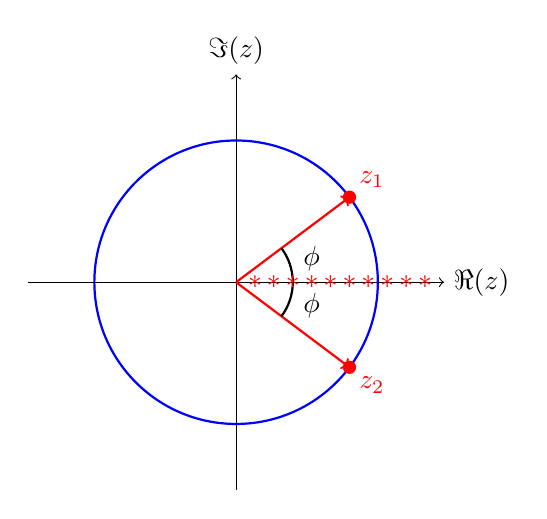
\begin{tikzpicture}[scale=1.2]
    \draw[->] (-2.2,0) -- (2.2,0) node[right] {$\Re(z)$};
    \draw[->] (0,-2.2) -- (0,2.2) node[above] {$\Im(z)$};
  
    \draw[thick,blue] (0,0) circle (1.5);
  
    \draw[->,thick,red] (0,0) -- (1.2,0.9);
    \draw[->,thick,red] (0,0) -- (1.2,-0.9);
    \fill[red] (1.2,0.9) circle (2pt) node[above right] {$z_1$};  
    \fill[red] (1.2,-0.9) circle (2pt) node[below right] {$z_2$};

    \draw[thick] (0.6,0) arc[start angle=0,end angle=36.87,radius=0.6]; 
    \node at (0.8,0.25) {$\phi$};
    \draw[thick] (0.6,0) arc[start angle=0,end angle=-36.87,radius=0.6]; 
    \node at (0.8,-0.25) {$\phi$};

    \foreach \x in {0.2,0.4,0.6,0.8,1.0,1.2,1.4,1.6,1.8,2.0}{
    \node[red] at (\x,0) {$\ast$};
    }
\end{tikzpicture}
\end{minipage}
\hfill
\begin{minipage}{0.5\textwidth}
\small
We have to consider the square root of a complex number $\sqrt{z}$, which is a multi-valued function:
\[
    \sqrt{z_1} = \sqrt{\rho} e^{i\phi/2}, \quad \sqrt{z_2} = \sqrt{\rho} e^{i(\phi/2 + \pi)} = -\sqrt{z_1},
\]
\[
    z_1 = \rho e^{i\phi}, \quad z_2 = \rho e^{i(2\pi-\phi)}.
\]
To ensure the function is single-valued, we introduce a branch cut along the positive real axis (indicated by red stars). The two roots \(z_1\) and \(z_2\) take on different values in the limits \(\phi \to 0\) and \(\phi \to 2\pi\), with \(z_2\) having a real part of opposite to that of \(z_1\):
\end{minipage}
\end{figure}
\[
    \sqrt{z_1} = \sqrt{\rho} \left[ \cos \frac{\phi}{2} + i \sin \frac{\phi}{2} \right], \quad \sqrt{z_2} = \sqrt{\rho} \left[ -\cos \frac{\phi}{2} + i \sin \frac{\phi}{2} \right].
\]
Thus we can express our integral in a complex variable \(p\), where we write \(p^2 + m^2 = (p+im)(p-im)\): 
\[
    A_{\mathbf{x} \to \mathbf{y}}(t) = I = \frac{-i}{(2\pi)^2 r} \int_{-\infty}^{\infty} \mathrm{d}p \, p e^{i p r} e^{-i \sqrt{(p+im)(p-im)}\, t}.
\]
\begin{figure}[H]
\centering
\begin{minipage}{0.45\textwidth}
\centering
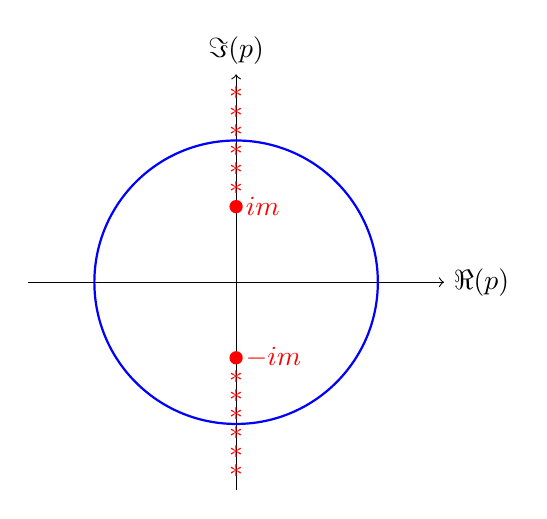
\begin{tikzpicture}[scale=1.2]
    \draw[->] (-2.2,0) -- (2.2,0) node[right] {$\Re(p)$};
    \draw[->] (0,-2.2) -- (0,2.2) node[above] {$\Im(p)$};

    \draw[thick,blue] (0,0) circle (1.5);

    \fill[red] (0.0,0.8) circle (2pt) node[right] {$im$};  
    \fill[red] (0.0,-0.8) circle (2pt) node[right] {$-im$};

    \foreach \x in {1.0,1.2,1.4,1.6,1.8,2.0}{
    \node[red] at (0,\x) {$\ast$};
    \node[red] at (0,-\x) {$\ast$};
    }
\end{tikzpicture}
\end{minipage}
\hfill
\begin{minipage}{0.5\textwidth}
\small
We have to consider the branch cuts starting from the branch points \(z = \pm im\) since both \(\sqrt{p + im}\) and \(\sqrt{p - im}\) are multi-valued functions with branch cuts defined along the imaginary axis (this time the discontinuities of the functions take place while crossing the imaginary axis). The branch cuts are indicated by red stars. We can now close the integration contour in the upper half-plane (the integrand vanishes in the limit \(|p| \to \infty\) in this half-plane).
\end{minipage}
\end{figure}
Using the Cauchy residue theorem, we can evaluate our integral by considering a contour that encloses the upper half-plane, avoiding the branch cut.
\[
    \int f(p)d\mathrm{p} = 2\pi i \sum \text{Res}(f, p_k) = 0, 
\]
since there are no poles inside the contour. The integral along the real axis is equal to the negative of the integral along the branch cut (the integral along the arc at infinity vanishes indeed):
\begin{figure}[H]
\centering
\begin{minipage}{0.5\textwidth}
\small
Let's denote the contour integral along the curve \(C\) as \(\oint_C f(p) \mathrm{d}p\). The contour \(C\) consists of three parts: the integral along the real axis from \(-\infty\) to \(\infty\), the integral along the two arcs at infinity in the upper half-plane (left and right of the branch cut), the integrals along the branch cut and the infinitesimal circulation around \(im\):
\[
    \int_{C_L} = -( \int_{C_1} + \int_{C_2} + \int_{C_{\epsilon}} + \int_{C_3} + \int_{C_4} ).
\]
\end{minipage}
\hfill
\begin{minipage}{0.45\textwidth}
\centering
\begin{tikzpicture}[scale=1.1]

    \draw[->] (-2.3,0) -- (2.3,0) node[right] {$\Re(p)$};
    \draw[->] (0,-0.5) -- (0,2.5) node[above] {$\Im(p)$};

    \foreach \y in {1.0,1.2,1.4,1.6,1.8,2.0, 2.2}{
      \node[red] at (0,\y) {$\ast$};
    }

    \draw[thick,red,<-] (0.2,0.8) arc[start angle=0,end angle=360,radius=0.2] node[right] {$C_{\epsilon}$};

    \draw[thick,->,green] (-2.2,0) -- (-1,0);
    \draw[thick,->,green] (-1,0) -- (1,0) node[below] {$C_L$};
    \draw[thick,green] (1,0) -- (2.2,0);

    \draw[thick,orange,
        postaction={decorate},
        decoration={markings, mark=at position 0.5 with {\arrow{<}}}
        ] (-2.2,0) arc[start angle=180,end angle=90,radius=2.2] node[above right] {$C_1$};

    \draw[thick,orange,
        postaction={decorate},
        decoration={markings, mark=at position 0.5 with {\arrow{>}}}
        ] (2.2,0) arc[start angle=0,end angle=90,radius=2.2] node[above left] {$C_4$};

    \draw[thick,->,blue] (0.1,2.2) -- (0.1,1.0) node[above right] {$C_2$};
    \draw[thick,<-,blue] (-0.1,2.2) -- (-0.1,1.0) node[above left] {$C_3$};

    \fill[red] (0,0.8) circle (2pt) node[right] {};  
    \fill[black] (-2.2,0) circle (2pt) node[below] {$-L$};  
    \fill[black] (2.2,0) circle (2pt) node[below] {$L$};  

\end{tikzpicture}
\end{minipage}
\end{figure}

We can now take the limit \(L \to \infty\) and \(\epsilon \to 0\). The integrals along the arcs at infinity vanish, and the integral around the infinitesimal circle \(C_{\epsilon}\) also vanishes.
\begin{enumerate}[label=(\roman*),align=left,itemsep=1.0\baselineskip]
    \item \textbf{Integral on the right arc at infinity vanishes}, \(\lim_{\vert p \vert \to \infty} \int_{C_1} f(p)\,dp = 0\):\\
    Outside the light cone (which is the only regime we are interested in), we can write:
    \[
        e^{ipr} e^{-it\sqrt{p^2 + m^2}} = e^{i \overline{\theta}} e^{-\Im(p)r} e^{t \Im(\sqrt{p^2 + m^2})} \to 0,
    \]
    as \(\vert p \vert \to \infty\) while mantaining \(r>t\). 
    
    \item \textbf{Integral on the left arc at infinity vanishes}, \(\lim_{\vert p \vert  \to \infty} \int_{C_4} f(p)\,dp = 0\):\\
    since:
    \[
        e^{ipr} e^{-it\sqrt{p^2 + m^2}} = e^{i \left[\Re(p)r - t\Re(\sqrt{p^2 + m^2}) \right]} e^{- \left[\Im(p)r + \left\vert \Im(\sqrt{p^2 + m^2}) \right\vert t \right]} \to 0,
    \]
    because we are on the left side of the branch cut, which imposes \(\Im(\sqrt{p^2 + m^2}) = - \vert \Im(\sqrt{p^2 + m^2}) \vert < 0\), thus the integral goes to zero as \(\vert p \vert \to \infty\).
    
    \item \textbf{Integral on infinitesimal circle vanishes}, \(\lim_{\epsilon \to 0} \int_{C_{\epsilon}} f(p)\,dp = 0\):\\
    From the Darboux inequality, we have:
    \[
        \vert \int_{C_{\epsilon}} f(p) \mathrm{d}p \vert \leq L_{C_{\epsilon}} \cdot \sup_{p \in C_{\epsilon}} \vert f(p) \vert,
    \]
    where \(L_{C_{\epsilon}} = 2\pi \epsilon\) and \(p \in C_{\epsilon} \implies p = im + \epsilon e^{i\theta}\) for \(\theta \in [0, 2\pi]\):
    \[
        \sup_{p \in C_{\epsilon}} \vert f(p) \vert = \frac{2\pi\epsilon}{(2\pi)^2 r} m e^{-mr} \sup_{\theta \in [0, 2\pi]} \left\vert e^{-it\sqrt{2im e^{i\theta}}} \right\vert \to 0 \quad \text{as } \epsilon \to 0.
    \]
    Since \(e^{-it\sqrt{2im e^{i\theta_{\text{max}}}}}\) is bounded for all \(\theta \in [0, 2\pi]\), this integral goes to zero as \(\epsilon \to 0\).
\end{enumerate}
We are thus left with an expression for the integrals on the real axis and the two sides of the branch cut:
\[    \int_{-\infty}^{\infty} f(p) \mathrm{d}p = -( \int_{C_2} + \int_{C_3} ) f(p) \mathrm{d}p.
\]
We are still considering the regime outside the light cone, \(r > t\). We can parametrize the two sides of the branch cut as follows: on the right side \(p = iy + \epsilon\) and on the left side \(p = iy - \epsilon\), with \(y \in [m, \infty)\) and \(\epsilon \to 0^+\). The integrals along the two sides of the branch cut can be compressed into a single integral\footnote{We use again the fact that on the left side of the branch cut, \(\sqrt{p^2 + m^2} = -\sqrt{y^2 - m^2}\) while on the right side \(\sqrt{p^2 + m^2} = \sqrt{y^2 - m^2}\).}:
\[
\begin{aligned}
    A_{\mathbf{x} \to \mathbf{y}} (t) &= \frac{i}{(2\pi)^2 r} \int_{m}^{\infty} \mathrm{d}y \, y e^{-yr} \left[ e^{t\sqrt{y^2 - m^2}} - e^{-t\sqrt{y^2 - m^2}} \right]\\
    &= \frac{i}{(2\pi)^2 r} \int_{m}^{\infty} \mathrm{d}y \, y e^{-yr} 2\sinh(t\sqrt{y^2 - m^2}).
\end{aligned}
\]
But we know that for \(y \geq m\) the integrand becomes a sum of positive or zero terms, thus the integral is non-zero:
\[
    y e^{-yr} 2\sinh(t\sqrt{y^2 - m^2}) \geq 0 \forall y \geq m \implies A_{\mathbf{x} \to \mathbf{y}} (t) \neq 0.
\]
Therefore, we have shown that even in a relativistic quantum mechanics framework, there is a non-zero probability of finding a particle outside the light cone, indicating a violation of causality. This violation is less pronounced than in non-relativistic quantum mechanics (since it is exponentially suppressed), but it still exists. This suggests that a more comprehensive framework is needed to fully reconcile quantum mechanics with the principles of special relativity, leading us to the development of quantum field theory.

\paragraph{Upper bound on \(\vert A_{\mathbf{x} \to \mathbf{y}} (t) \vert\).} We can also derive an upper bound for the amplitude outside the light cone. Starting from the expression:
\[
\begin{aligned}
    \sinh(t\sqrt{y^2 - m^2}) < e^{t\sqrt{y^2 - m^2}} < e^{yt},\\
    \implies \vert A_{\mathbf{x} \to \mathbf{y}} (t) \vert < \frac{1}{(2\pi)^2 r} \int_{m}^{\infty} \mathrm{d}y \, y e^{-y(r - t)} = \frac{1}{(2\pi)^2 r} \frac{m(r - t) + 1}{(r - t)^2} e^{-m(r - t)}.
\end{aligned}
\]
This upper bound shows that the amplitude decreases exponentially with the distance \(r\) outside the light cone, modulated by a polynomial factor. This indicates that while causality violations are present, they become increasingly unlikely as one moves further away from the light cone, especially for larger values of the particle mass \(m\).

\section{Towards Quantum Field Theory}